\begin{figure}[h]
	 \centering	
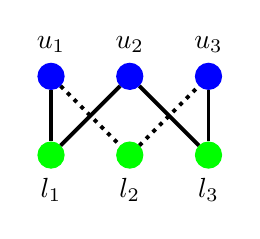
\begin{tikzpicture}
	\node[shape=circle,draw=blue,fill=blue,label=above:$u_1$] (1) {};
	\node[shape=circle,draw=blue,fill=blue,label=above:$u_2$] (2) [right of=1] {};
	\node[shape=circle,draw=blue,fill=blue,label=above:$u_3$] (3) [right of=2] {};
	\node[shape=circle,draw=green,fill=green,label=below:$l_1$] (4) [below of=1] {};
	\node[shape=circle,draw=green,fill=green,label=below:$l_2$] (5) [below of=2] {};
	\node[shape=circle,draw=green,fill=green,label=below:$l_3$] (6) [below of=3] {};

	\draw (1) [line width=0.5mm] -- (4);
	\draw (1) [dotted,line width=0.5mm] -- (5);
	\draw (4) [line width=0.5mm] -- (2);
	\draw (5) [dotted,line width=0.5mm] -- (3);
	\draw (6) [line width=0.5mm] -- (3);
	\draw (6) [line width=0.5mm] -- (2);
\end{tikzpicture}

\caption{Example of \acrshort{bt} in \acrshort{bg}}
\label{fig:bitriangle-example}
\end{figure}

	